\documentclass[12pt]{article}

\usepackage{scicite,times,graphicx,float,hyperref}
\usepackage[skip=0pt]{caption}
\usepackage[utf8]{inputenc}
\usepackage{enumitem}
\usepackage{booktabs}

%%%%%%%%%%%%%%%%%%%%%%%%%%%%%%%%%%%%%%%%%%%%%%%%%%%%%%%%%%%%%%%%%%%%%%%%%%% PREAMBLE %%%%%%%%%%%%%%%%%%%%%%%%%%%%%%%%%%%%%%%%%%%%%%%%%%%%%%%%%%%%%%%%%%%%%%%%%%%

\topmargin -1.0cm
\oddsidemargin 0.0cm 
\textwidth 16cm 
\textheight 23cm
\footskip 1.0cm

\newenvironment{sciabstract}{%
\begin{quote} \bf}
{\end{quote}}

\newcounter{lastnote}
\newenvironment{scilastnote}{%
  \setcounter{lastnote}{\value{enumiv}}%
  \addtocounter{lastnote}{+1}%
  \begin{list}%
  {\arabic{lastnote}.}
  {\setlength{\leftmargin}{.22in}}
  {\setlength{\labelsep}{.5em}}
}
{\end{list}}

\title{Intermediate Report on:\\Pretix Cluster Deployment \& Management} 

\author
{Filipe Pires [85122], João Alegria [85048]\\
\\
Computational Infrastructures Management\\
\normalsize{Department of Electronics, Telecommunications and Informatics}\\
\normalsize{University of Aveiro}\\
} 

\date{\today{}}

%%%%%%%%%%%%%%%%%%%%%%%%%%%%%%%%%%%%%%%%%%%%%%%%%%%%%%%%%%%%%%%%%%%%%%%%%%%% REPORT %%%%%%%%%%%%%%%%%%%%%%%%%%%%%%%%%%%%%%%%%%%%%%%%%%%%%%%%%%%%%%%%%%%%%%%%%%%%

\begin{document} 

\baselineskip18pt

\maketitle 

\section*{Introduction} \label{introduction} %%%%%%%%%%%%%%%%%%%%%%%%%%%%%%%%%%%%%%%%%%%%%%%%%%%%%%%%%%%%%%%%%%%%%%%%%%%%%%%%%%%%%%%%%%%%%%%%%%%%%%%%%%%%%%%%%%%

This report aims to describe the work developed for the intermediate phase of the practical assignment of the discipline of Computational Infrastructures 
Management \cite{assign} from the Msc. degree in Informatics Engineering of the University of Aveiro at the Department of Electronics, Telecommunications and 
Informatics.
It is here included:
a product description and the respective expectations regarding client capacity, derived from a thorough analysis;
the adopted clustering strategy, considering matters such as virtualization, storage, network and load distribution mechanisms;
an explanation of the performance analysis executed based on the department's support platform for representative use cases;
and the results drawn from such analysis, to be considered during the second phase of development.

The service provided is Pretix, an online shop, box office and ticket outlet already successfully used by other service providers for conferences, festivals, 
exhibitions, workshops and more.
All code developed is publicly accessible in our GitHub repository:

\url{https://github.com/FilipePires98/GIC}.

\newpage
\section{Pretix Ticketing Software} \label{pretix} %%%%%%%%%%%%%%%%%%%%%%%%%%%%%%%%%%%%%%%%%%%%%%%%%%%%%%%%%%%%%%%%%%%%%%%%%%%%%%%%%%%%%%%%%%%%%%%%%%%%%%%%%%%%%

% what is pretix?

Pretix \cite{pretix} is an all-in-one product, serving as an online shop, box office and ticket outlet, meant for companies that aim to host events of numerous kinds.
This ticketing software created by Rami.io \cite{rami.io} has a wide variety of features that range from ticket shop customization (domain definition, multiple 
language support, product structure with multiple categories, packages and possibility for donations, seating plans, website embeddings, etc.) and marketing 
(voucher system, email, campaign tracking, etc.), to payment definition (invoicing and multiple payment methods) and on-site management (check-in lists, ticket 
scans, etc.), and even administrative control (with statistics and event-spanning reports, team permissions and data export and API).

As a complete solution, Pretix has already been successfully used for conferences, festivals, concerts, shows, exhibitions, workshops, barcamps, and more 
according to the creators.
The software's source code is completely open \cite{pretixgit}, and the authors make available extensive documentation \cite{pretixdoc}, an installation 
guide and a support blog.

\subsection{Our Product} \label{pretix.product} %%%%%%%%%%%%%%%%%%%%%%%%%%%%

% what is our purpose? what are we offering?

What we offer, as a developers team, is the Pretix' infrastructure deployment and management as a service that could potentially be provided to businesses 
interested in hosting events by taking advantage of Pretix' many advantages, without having resources or knowledge of how to deploy it themselves.
Our contract is simply to ensure the correct, reliable, secure and constant functioning of Pretix, capable of supporting usage scenarios of the same magnitude 
as of the one described next.

\subsection{Use Case Scenario} \label{pretix.scenario} %%%%%%%%%%%%%%%%%%%%%

% what do we intend to be able to support?
% how many users and/or requests per second is the system supposed to be able to handle?

In order to ensure the fulfillment of our contract, a representative scenario of usage was defined to guide us throughout development.
A simulated organization intends to host a WebSummit-like event by the end of this year.
It has analysed the feature list of Pretix and wishes to adopt it in the future.
However, as it is its first time using the software, the company decided to use it simply as a ticket purchase platform and reduced the payment methods to 
on-site manual payment only. 
The organization expects to sell 10 000 tickets in a week and warned us that in previous events they witnessed a peak close to the end of the selling period.

In practical terms this means that we only need to concern ourselves with the online ticket purchasing features and do not even need to consider the actual 
payment process, although it was our intent from the beginning to support most of Pretix's features even if most would not be used.
It also means that we had to build the system considering our hardware limitations and the activity peak expectation.

\subsection{Support Requirements} \label{pretix.requirements} %%%%%%%%%%%%%%

% what components need to exist for the product to be fully supported?
% what are the minimal hardware requirements for its deployment?

As stated in their documentation, to use Pretix it is required:
\vspace{-10pt}
\begin{itemize}[noitemsep]
  \item Pretix and the python packages it depends on
  \item An WSGI application server
  \item A periodic task runner
  \item A database
  \item A reverse proxy
  \item A server for caching, session storage and task queuing
\end{itemize}
\vspace{-10pt}
As we intended to deploy the product in containers, Docker became an additional requirement.

Regarding the hardware remotely available at our department, it was allocated for us an infrastructure of a total of 58 nodes and 115 cores, with 5.6TB of 
storage and 235.8GB of RAM available.
However, this is destined for several developer teams, meaning that we must only use a small portion of such resources, by our estimates of less than 10\% of 
the total capacity.

Also according to Pretix' documentation, the software has some scalability limitations.
In some cases their software needs to "fall back to event-global locking for some actions which are likely to run with high concurrency and cause harm".
For every event, only one of such locking actions can be run at the same time.
With this in mind, they estimate a maximum capacity of approximately 500 orders per minute per event, "even if you add more hardware".
However, they also mention that if the event to be hosted has an unlimited number of tickets (which is our case), fewer locking is applied and thus it is 
possible to reach approximately 1500 orders per minute per event.

Considering all of these aspects, we made an estimation of how many ticket purchase requests we would be able to support per minute.
At this preliminary stage, we believed it could be achieved a capacity of 800 ticket purchases per minute without a relevant amount of failed attempts.
In chapter \ref{performance} we explore our own system in an attempt to determine whether our estimations were correct and feasible or not.

%\texttt{java -cp <userdir>/build/classes fi.FarmInfrastructure}

% \vspace{-10pt}
% \begin{itemize}[noitemsep]
%   \item ...
% \end{itemize}
% \vspace{-10pt}

% \vspace{-10pt}
% \begin{enumerate}[noitemsep]
%   \item ...
% \end{enumerate}
% \vspace{-10pt}

% \begin{figure}[H]
%   \centering
%   \begin{minipage}{\textwidth}
%     \centering
%     \includegraphics[width=\linewidth]{img/.....png}
%   \end{minipage}%
%   \caption{...}
%   \label{...}
% \end{figure} 

\newpage
\section{Clustering Strategy} \label{strategy} %%%%%%%%%%%%%%%%%%%%%%%%%%%%%%%%%%%%%%%%%%%%%%%%%%%%%%%%%%%%%%%%%%%%%%%%%%%%%%%%%%%%%%%%%%%%%%%%%%%%%%%%%%%%%%%%%

\subsection{Deployment Architecture and Service Decomposition} \label{strategy.architecture} %%%%%%%%%%%%%%%%%%%% 

% what are the dependencies? what components does the cluster have?

Docker \cite{docker} allows us to deliver the infrastructure in isolated containers with well-defined communication channels.
This dramatically reduces infrastructure resources required and facilitates its management, while ensuring consistency within the whole environment.
Also, its simplicity in configurations and rapid deployment makes it perfect for its use in any system with a reasonably large size and complexity.

By taking advantage of Pretix' support for Docker, its dependencies were covered after analyzing which technologies would be most appropriate for our scenario.
With an already fully functional Docker Image publicly available \cite{pretix_img}, the authors of the product made the deployment of the web application easier.
In it is the Django-based \cite{django} web application that provides all the services and resources of Pretix, an instance of Gunicorn \cite{gunicorn}, a 
Web Server Gateway Interface (WSGI) hosting the application, and lastly an instance of NGinX \cite{nginx}, a reverse-proxy for the web application deployment 
in production mode - this last component is needed because the Django framework, when in production, divides the static resources and the dynamic resources and 
worries only about the dynamic ones, assuming that a reverse-proxy serves de static ones. 
Pretix' container configuration file also simplified the connection between the product and the storage containers, namely for the required database and caching server.

To handle all storage we chose PostgreSQL \cite{postgresql}.
This relational Database Management System (DBMS) had powerful tools to deal with scalability and redundancy, so it was quickly understood as a good option, 
although others like MariaDB were strongly considered as well.
It is the PostgreSQL that stores the data related to organizations, events, tickets, clients, invoices, etc.
In our case a PostgreSQL cluster is instantiated for redundancy purposes in a Master-Slave mode.
Currently, a single PostgreSQL master and 2 slave nodes are instantiated, and if the master fails the system is capable of assigning one of the slaves as the 
new master.

A similar approach was followed for the caching server.
This server has the responsibility of storing in-memory relevant data such as open user sessions, live events, etc. and of asynchronously queuing tasks.
In this case, the chosen tool was Redis \cite{redis}, instantiated in a Master-Slave cluster mode with 1 master and 2 slave nodes as well. 
The failover process is also supported with the help of sentinels. 
Sentinels are nodes natively supported by redis which have the responsibility of over-watching / taking care of the cluster and in case any change occurs, 
such as the addition or removal of a (slave or master) node, it registers that modification and notifies the necessary nodes so that they can reconfigure themselves. 
In our case we opted to instantiate two sentinels. \\

A problem encountered during the infrastructure configuration was that if a master node crashed in one of the storage clusters, the connection to the storage 
infrastructure was lost since the association to the cluster is through it's master(s).
With the master machine down in a distributed environment, the service was incapable of locating the new master. 
This and the efforts applied in balancing the load to the service forced us to add a proxy for both clusters.

Pgpool \cite{pgpool} was introduced to solve the problem for the PostgreSQL cluster. 
This middleware works between PostgreSQL servers and clients and enables connection pooling, replication, load balancing and more, although we used only the first
3 features.
This component served as a proxy that, when connected to, always redirects requests to the master of the PostgreSQL cluster and, if there was more than 1 master, 
the requests would be distributed in a balanced way over the available masters. 

For the Redis cluster, an HAProxy \cite{haproxy} was found to be the best option for our scenario, since it provided us a reliable and high performing load balancer.
This component, similarly to the one mentioned above, works as a proxy that forwards requests to one of the cluster masters, balancing the load in case there 
are severel master nodes.

The last component of our architecture is a reverse-proxy of our own, implemented using NginX, with the aim to balance the requests made to the Pretix service itself. 
This component, as suggested by the name reverse-proxy, also enabled us to access multiple instances of the Pretix server through a unique endpoint, facilitating 
the interaction between clients and service.

\begin{figure}[H]
  \centering
  \begin{minipage}{.85\textwidth}
    \centering
    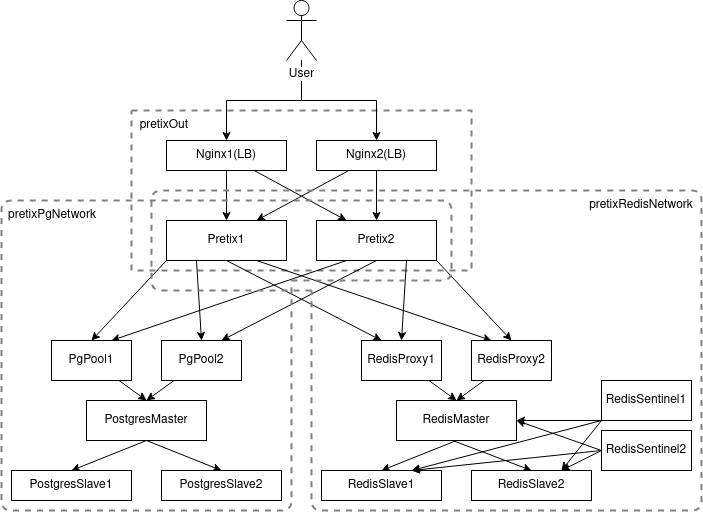
\includegraphics[width=\linewidth]{diagrams/InfrastructureArchitecture.png}
  \end{minipage}%
  \caption{Infrastructure architecture diagram deployed in Docker Swarm.}
  \label{fig:InfrastructureArchitecture}
\end{figure}

To provide this service we focused on some aspects that we considered paramount: availability, consistency, maintainability, scalability, redundancy, fault 
tolerance and load balancing. 
Those were the quality attributes we were looking to achieve when making every service redundant (by having replicas or through clusters), and when implementing 
the storage infrastructures as clusters and the mentioned proxies (for the storage systems and the service itself).
The result is visible in Figure \ref{fig:InfrastructureArchitecture}.

\subsection{Deployment} \label{strategy.deployment} %%%%%%%%%%%%%%%%%%%%%%%%

% how exactly is the system being deployed?

For this project there are 2 methods available to deploy the service stack: in a traditional Docker deployment through the usage of Docker Compose or in Docker 
Swarm mode.
The intended method was the second one, since the powerful infrastructure hosted in the DETI's department was made available for all groups. 
However, it was implemented not only a stack deployment for Docker Swarm but also one for the normal Docker Compose, since the second could be used for testing 
purposes. 
Both implementations respect our architecture but are naturally deployed with some differences in configurations, since each mode supports different features.

An experimentation phase occurred when searching for the best available solutions and containers that would suit our needs.
This in itself was quite a challenge, but the integration process of all containers proved to be far more challenging and complex than previously presumed.
The final version uses the following images from Docker Hub:
\vspace{-10pt}
\begin{itemize} [noitemsep]
  \item PostgreSQL Master/Slave: \href{https://hub.docker.com/r/bitnami/postgresql-repmgr}{https://hub.docker.com/r/bitnami/postgresql-repmgr}
  \item PostgreSQL Pool(PgPool): \href{https://hub.docker.com/r/bitnami/pgpool}{https://hub.docker.com/r/bitnami/pgpool}
  \item Redis Master/Slave/Sentinel: \href{https://hub.docker.com/\_/redis}{https://hub.docker.com/\_/redis}
  \item Redis Proxy: \href{https://hub.docker.com/\_/haproxy}{https://hub.docker.com/\_/haproxy}
  \item Pretix: \href{https://hub.docker.com/r/pretix/standalone}{https://hub.docker.com/r/pretix/standalone}
  \item NginX: \href{https://hub.docker.com/\_/nginx}{https://hub.docker.com/\_/nginx}
\end{itemize}
\vspace{-10pt}
Obviously, some of these images serve only as a base for self created images. 
This was desirable because in certain situations we needed a higher degree of control (e.g. for a container to wait for other containers to start first). 
This necessity for self-created images happened with: the Redis Slave image, to configure the Redis server to be a slave of a given machine and wait for the 
cluster master; the Redis Sentinel, to configure the Redis server to behave as a sentinel of the cluster and wait for the cluster master; the Redis Proxy, to 
configure the HAProxy so that the proxy would have in consideration all redis nodes and always access the master; and with Pretix itself, for the container 
to wait for the PostgreSQL and the Redis Proxies.

With each component defined, the stack was divided logically in 3 networks: each cluster belongs to one of the networks, NGinX has its own network, and the 
Pretix service is the linking element between the 3 networks.
This is also represented in Figure \ref{fig:InfrastructureArchitecture}.

Another aspect that we took in consideration was the data produced by the application itself. 
We needed a consistent and fault-tolerant system, so the data produced could not be lost under no circumstances. 
So volumes were assigned to the containers so that no information was lost, even if all services crashed.
All volumes were defined and mounted in a Network File System (NFS) provided \textit{a priori} for the discipline.

Lastly, some configuration files needed to be injected into containers, namely the Pretix server and the NginX reverse-proxy. 
To do this, we resort to the so called secrets: in our stack definition file, those configuration files were defined as secrets along with their destinations; 
such secrets are then generated automatically when the stack is deployed. 

Both Docker Compose and Docker Swarm accept the same stack configuration file. 
This is quite useful as it avoided duplicated work.
Nevertheless, as we have mentioned, there are significant differences between the 2 deployment methods, that in practical terms translates to certain fields 
being present in a mode and not in the other, namely the \texttt{deploy}, \texttt{configs} and \texttt{secrets} fields that are not processed in the Compose mode.
This meant that the automatic replication provided by Swarm is not available as well as the inject of configuration files and secret files. 
And since we mostly debugged and tested locally with Docker Compose, we felt the need to create an auxiliary stack configuration file that would deploy the 
system that basically replicates the one in Swarm. 
In this file, the only changes were: the mounting point for the volumes (as this configuration was not intended to be deploy in the remote infrastructure); the 
replication (manually defined by creating different containers); and the configuration files otherwise injected by secrets API (now injected as volumes). Furthermore, a simplification was made since the Compose replication was made manually; in Compose we deployed with the minimum replication and redundancy, meaning that we only had one replica of each service: the clusters consists of 1 master and 2 slaves, the proxies and the main server have only 2 replicas, where in Swarm we had at least three instances of a service, clusters were kept the same, proxies with 3 replicas and the service with 5 replicas(since it is the most important component and the one assumed to be the bottleneck in the stack).

A last remark needs to be made related to the deployment section and the reason behind some practical decisions and configurations we made. We already explained the reasons behind our deployment architecture and service decomposition, such as the implementation of clusters and replication of services to increase the fault tolerance, availability, consistency, etc. But in the Swarm stack configuration file there are two distinct ways of replicating a service, using the replication feature provided by Swarm itself and replicated manually, such as the slaves in the PostgreSQL cluster. This difference is caused purely by practical limitations; the solution used for the PostgreSQL cluster needs nodes with different configurations, and consequently different services to accommodate those configurations. This limitation  was tested by ourselves. The remaining services are configured so that a direct replication is possible.

In this delivery, the number of replications and cluster sizes were conservative since the intent is to make a proof of concept and learn more about the service provided and the constraints it has. In further work we intend to increase these values as necessary.

\subsection{Distribution} \label{strategy.distribution} %%%%%%%%%%%%%%%%%%%%

% how exactly is the system being distributed?

Docker Swarm not only adds some quite important features in the quality assuring realm (replication, load balancing, etc.), but it does that in a distributed way. 
This allows the Swarm mode to spread across as many machines as the user wants. 
The provided remote infrastructure is spread across 3 machines, each with several virtual machines created so that the swarm has more agents to use and thus 
simulating a truly heterogeneous and distributed environment.

Because we deploy our service stack in the Docker Swarm established in the remote infrastructure, our stack was distributed by design, which was one of the 
characteristics that appealed us in the beginning. 
This basically means that independently of the available machines, the number of machines, their operational system, their location, and so on, installing docker 
on all of them and establishing the Swarm mode across all, safely guarantees that the stack can be deployed in such scenario and it will work just as expected.

Through the usage of the provided platform, we concluded that the distribution is made automatically by assigning a task to an agent. 
A task is normally a replica of a service and the agent is a machine running a docker daemon somewhere in the Swarm network. 
Since each service consists in one or more replicas, they are spread across the Swarm network as the platform finds fit.
This distribution is quite important since it enables the user to gain access to the power of not only one machine, but all those assigned to tasks of his stack, 
making possible smaller response times. 
This does not happen when a local deployment with Docker Compose is made, since this approach uses only one machine for all services needed, overloading all 
computational resources and thus increasing the response times.

However, no solution is perfect and this is no exception.
While locally the bottleneck is clearly CPU and RAM capacity, in an infrastructure such as the one provided in the department additional factors play a role in 
the overall performance, namely the communication speed amongst machines and the networks' bandwidths available.
The ideal solution is one where these aspects have a capacity proportional to the processing capacity of the machines themselves, but as we will see further 
ahead this unfortunately isn't quite the reality.

\newpage
\section{Current Cluster Performance} \label{performance} %%%%%%%%%%%%%%%%%%%%%%%%%%%%%%%%%%%%%%%%%%%%%%%%%%%%%%%%%%%%%%%%%%%%%%%%%%%%%%%%%%%%%%%%%%%%%%%%%%%%%%

% what was done to evaluate its current performance?

In order to determine the true capacity of our deployed solutions, a set of measures were performed both locally and on the remote, shared and more powerful 
infrastructure.
Although replication and redundancy were already concerns of ours, we were not yet focused on determining availability statistics.
Rather, our aim was to test our services in terms of load capacity.

We wished to determine how many users were supported simultaneously accessing Pretix and attempting to purchase tickets to our fictitious event.
To do this, we performed benchmarking tests and tracked the number of failures both in the act of requesting a purchase and in the act of storing purchases in 
our databases.
In this chapter we describe the efforts made for benchmarking and the bottlenecks discovered from our performance evaluation.

\subsection{Benchmarking} \label{performance.benchmarking} %%%%%%%%%%%%%%%%%

% what framework was used for load testing and how was it used?

After doing research on available tools and frameworks, we reached the conclusion that the most adequate would be Locust \cite{locust}.
Locust is an open source, intuitive, distributed, user load testing framework intended to "figure out how many concurrent users a system can handle" by 
programmatically simulating thousands of users called locusts.
During tests, systems are "attacked" by a swarm of locusts whose behavior is defined by the developer in Python and the swarming process is monitored from a 
web UI in real-time. 

When defining the behavior of our locusts, some considerations had to be dealt with.
The job of a locust wasn't simply to send an HTTP request to purchase a ticket; real users need to go through a purchasing process on Pretix' web platform, and 
in that process the user's browser requests far more data from the server than the mere purchase action.
So this process needed to be somehow simulated as well.
Several possibilities were considered to achieve this.

Selenium \cite{selenium}, a suite of tools for automating web browsers, is a widely used solution for testing purposes; however, we intended to launch thousands 
of virtual users and so, even with options such as launching browsers in headless mode (without rendering page elements), this created a bottleneck of processing 
elements that were not relevant to us and did not represent the true capacity of the system, thus rendering the whole benchmark invalid.
Other alternatives like wrappers to drive browsers in Python were tried but proved to be too limited for our purposes.

The solution was to manually go through the purchase process once on the Pretix website and collect all network requests that were being made, including CSS 
resources, image files, Javascript code and requests sent to Pretix' REST API.
Amongst these requests was the actual purchase action in a message of type POST.
Then, we replicated all requests on the locust behavior and, by reading Pretix' API documentation, were able to manipulate the POST request to seem to come 
from different users.
We also included optional data on such requests, like invoices, to increase the load the server needed to process and so establishing a worst-case-scenario usage 
that would give us more comfort regarding the faithfulness of the results.

\subsection{Execution} \label{performance.execution} %%%%%%%%%%%%%%%%%%%%%%%

% how was the benchmarking done?

Having established the behavior of the fictitious users, we proceeded to actually executing our benchmarking.
This was divided in 2 groups of tests of 4 phases each.
The first group was entirely performed locally in one of our personal computers, the second was performed remotely using our Docker Swarm.
This was done in order to clearly comprehend the differences of performance between the 2 deployment methods and detect which bottlenecks were common to both 
and which appeared only in the second group (if any).

The 4 phases consisted in load testing the solution with 4 different activity peaks: one with half the expected load, one with the expected load, one with 
twice as many expected users and one with 10 times as many users.
These were defined a priori and the expected load was set according to the analysis described in section \ref{pretix.requirements}. 

% It is important to mention that some failed requests were treated in a particular manner after reflecting on the issue.
% This is the case for accessing requests to the ticket purchase root path and for completing a purchase process.
% In these situations the fictitious user attempts to successfully execute them 3 times.
% This was decided after considering that in reality, an interested client would not mind to have to reload a page in the event it failed the first time, even more 
% if this would occur in the completing action of the ticket purchase.
% Although this naturally improved the results, all failures were considered in our overall evaluation.
% Failures are here distinguished from 3-times failures by naming the later as exceptions. \\

The results of the first group of tests are presented next.
For the local tests it is important to consider the hardware used and its activity in stand-by.
It was used a computer with 12Gb of RAM and 8 CPU cores; before any tests were executed, 1 thread was running with CPU at 10\% of its capacity and around 6Gb 
of memory being used.
Each phase was executed 5 times, so the values here presented are always an average of such executions in order to remove potential noise from the results.

The first locust swarm attacked the service with 400 clients, with a hatch rate of 20 per second (the maximum rate found for the hardware to handle).
The attack took about 1 minute and 26 seconds, with the swarm complete 34 seconds after initialization.
The average response time of all API requests aggregated was 737ms (with the fastest being 3ms and the slowest response taking 50278ms).
Over 22000 requests were made in that period, with only 3 failures corresponding to POST requests of the actual purchasing final action (henceforward referred
to as order-post).
This means that, of the 400 users that attempted to purchase a ticket to our event, 3 of them were unable to do so, resulting in a success rate of 99.25\%.
Note that during this test the computer maintained all cores working at around 70\% capacity and the memory reached a maximum peak of 9.63Gb.

For the second locust swarm, 800 clients were hatched - our target number - at the same rate as before.
The attack duration was of 2 minutes and 32 seconds, with the swarm complete after around 1 minute of execution.
The aggregate response times almost duplicated at an average of 1700ms, although for the order-post only raised from 1000ms to 1300ms.
Under this scenario the amount of errors kept the same, resulting in a success rate of 99.625\%.
Hardware usage was very similar to the first phase, with a slight increase in memory usage to 9.87Gb.

In the third phase the infrastructure behaved as expected.
Amongst the 1600 users hatched, 6 of them were unable to purchase a ticket.
Response times increased to an average of 3000ms both aggregated and on the order-post, with some users having to wait almost 2 minutes for the order completion.
CPU usage kept steady at 70\% and RAM increased to 10.0Gb.
This phase took over 6 minutes, with the 100th user hatched after 2 minutes of execution.

The fourth and final phase was by far the slowest, although its results were positive.
We realized from the beginning that these tests would be compromised by the hardware hosting them, but this was specially true when attempting to test 8000 
simultaneous user.
Hatching them took over 10 minutes and their execution lasted for almost 40 minutes.
Memory was completely used at about 10.8Gb making the 8 threads suffer from "hiccups".
From the 8000 users, 37 were unable to purchase a ticket, but many of those that were able had to wait over 15 minutes to do so, which would be completely 
unacceptable in a real case scenario.

\begin{figure}[H]
  \centering
  \begin{minipage}{\textwidth}
    \centering
    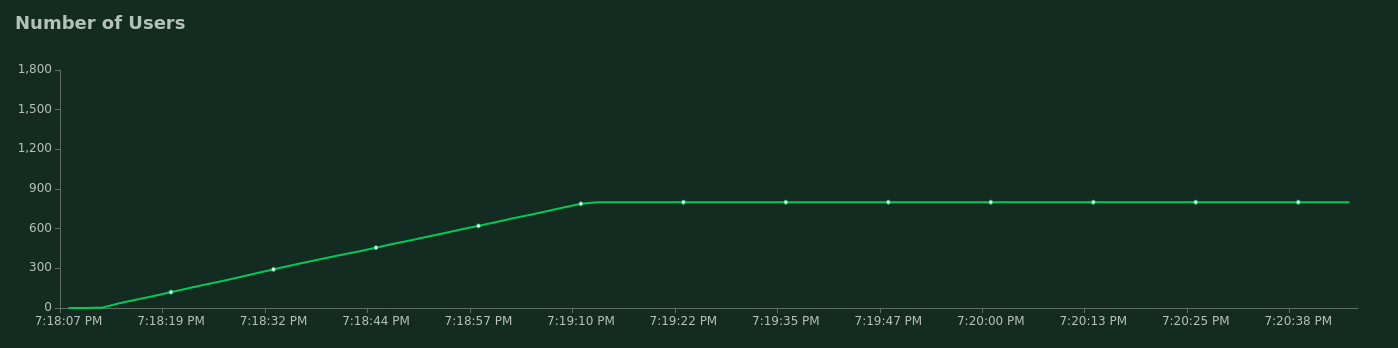
\includegraphics[width=\linewidth]{tests/local/800/number_of_users_1588097887.png}
  \end{minipage}%
  \label{fig:LocalTests:number_of_users}
  \begin{minipage}{\textwidth}
    \centering
    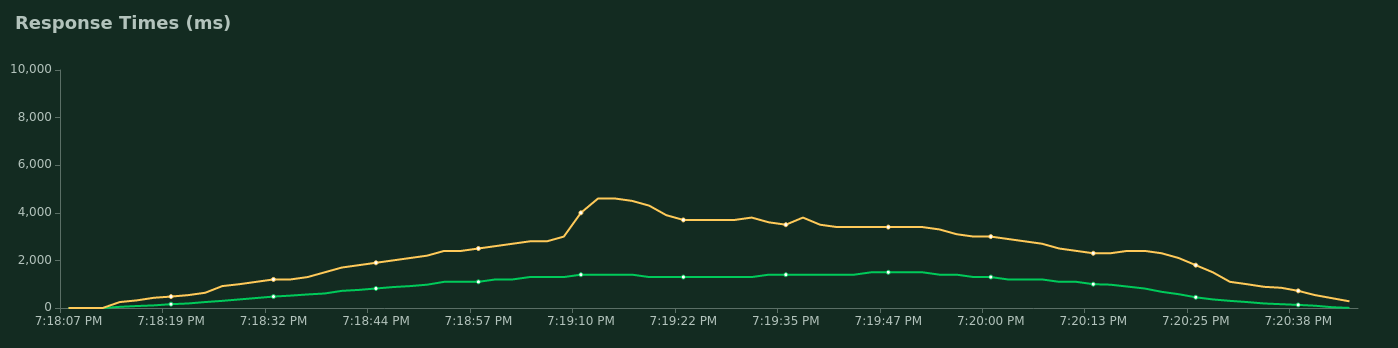
\includegraphics[width=\linewidth]{tests/local/800/response_times_(ms)_1588097887.png}
  \end{minipage}%
  \label{fig:LocalTests:response_times_(ms)}
  \begin{minipage}{\textwidth}
    \centering
    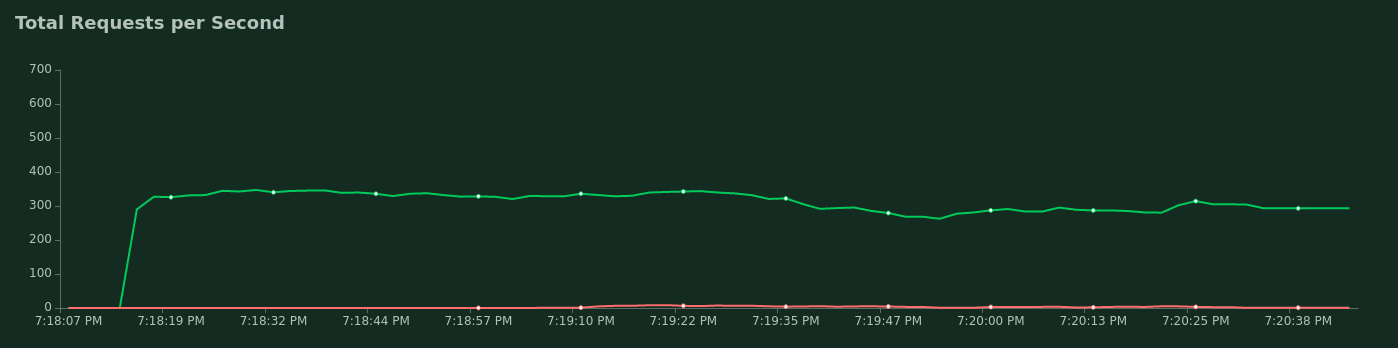
\includegraphics[width=\linewidth]{tests/local/800/total_requests_per_second_1588097887.png}
  \end{minipage}%
  \caption{Load tests results with 800 users.}
  \label{fig:LocalTests:total_requests_per_second}
\end{figure}
\vspace{-10pt}

Figure \ref{fig:LocalTests:total_requests_per_second} contains 3 graphics taken from Locust's web UI, with the first corresponding to the number of hatched 
users over time, the second to the response times in milliseconds (green line is the median values, yellow is in 95\% percentile), and the total requests per
second (with the red line corresponding to failures).

%%%%%%%%%%%%%%%%%%%%%%%%%%%%%%%%%%%%%%%%

% https://docs.pretix.eu/en/latest/api/fundamentals.html
% Responses with status code 409 Conflict are not cached. If you send the request again, it will be executed as a new request, since these responses are intended to be retried.

%%%%%%%%%%%%%%%%%%%%%%%%%%%%%%%%%%%%%%%%

% 0
% 0/s

% Mem 7.4Gb / 11.6Gb
% 8 cores at ~10\%
% 1 thr running

%%%%%%%%%%%%%%%%%%%%%%%%%%%%%%%%%%%%%%%%

% 400
% 20/s

%  (start),  (all users),  (end)

% Mem 9.63Gb / 11.6Gb
% 8 cores at ~70\%
% 8 thr running

% Type 	Name 	                                        # Requests 	# Fails   # Exceptions  Median (ms) 	90%ile (ms) 	Average (ms) 	Min (ms) 	Max (ms)
% POST 	/api/v1/organizers/ws/events/ws2020/orders/ 	456 	      59 	      3             810 	        1500 	        1024 	        150 	    11199
%       Aggregated                                    22435       59        -             610           990           737           3         50278 

%%%%%%%%%%%%%%%%%%%%%%%%%%%%%%%%%%%%%%%%

% 800
% 20/s

% Mem 9.87Gb / 11.6Gb
% 8 cores at ~70\%
% 8 thr running

% Type 	Name 	                                        # Requests 	# Fails   # Exceptions  Median (ms) 	90%ile (ms) 	Average (ms) 	Min (ms) 	Max (ms) 
% POST 	/api/v1/organizers/ws/events/ws2020/orders/ 	906 	      109 	    3             1300 	        1800 	        1325 	        165 	    8682 	
%       Aggregated                                    44885       369       -             1100          1700          1343          2         83344 

%%%%%%%%%%%%%%%%%%%%%%%%%%%%%%%%%%%%%%%%

% 1600
% 20/s

% Mem 10.0Gb / 11.6Gb
% 8 cores at ~70\%
% 8 thr running

% Type 	Name 	                                        # Requests 	# Fails   # Exceptions  Median (ms) 	90%ile (ms) 	Average (ms) 	Min (ms) 	Max (ms) 
% POST 	/api/v1/organizers/ws/events/ws2020/orders/ 	1772 	      178 	    6             1800 	        3200 	        2904 	        173 	    121762
%       Aggregated 	                                  89730 	    1426 	    -             1400 	        3200 	        3232 	        2 	      181509

%%%%%%%%%%%%%%%%%%%%%%%%%%%%%%%%%%%%%%%%

% 8000
% 20/s

% Mem 10.8Gb / 11.6Gb
% 8 cores at ~70\%
% 8 thr running

% Type 	Name 	                                        # Requests 	# Fails   # Exceptions  Median (ms) 	90%ile (ms) 	Average (ms) 	Min (ms) 	Max (ms)
% POST 	/api/v1/organizers/ws/events/ws2020/orders/ 	9177 	      1214 	    37            2700 	        5000 	        15635 	      62 	      1022473 
%       Aggregated 	                                  448918 	    10898 	  -             1900 	        4600 	        20335 	      2 	      1579377 

%%%%%%%%%%%%%%%%%%%%%%%%%%%%%%%%%%%%%%%%

With the system fully deployed using Docker Swarm, the second group of tests was performed, and their results are presented next.
Note that the machine running these tests had a different capacity than that of the local tests, running Ubuntu 18.0.4 with 2 CPUs and 4Gb of RAM (the reason 
for this is explained in section \ref{performance.bottlenecks}).
As it was a remote machine, the monitoring of its behavior was very limited.

The first swarm attacked the service with 400 clients, with a hatch rate of 20 per second.
The attack took about 5 minutes and 20 seconds, with the swarm complete around 30 seconds after initialization.
This compared to the local tests was already very different, with a delay of 4 minutes.
The average response time of all API requests aggregated was 5767ms
About the same number of requests were made as the ones from the local tests, with a discouraging amount of order-post failures reaching 178.
This means that, of the 400 users that attempted to purchase a ticket to our event, almost half of them (44.5\%) were unable to do so.
Additionally, the \texttt{409 Conflict} (see section \ref{performance.bottlenecks} for more on this error) was not the only error message returned, meaning that 
this percentage was in fact much higher due to errors of type \texttt{502 Bad Gateway}, \texttt{504 Gateway Timeout} and the more generic type 
\texttt{500 Internal Server Error}.
We had reached the maximum response capacity of the system with half the users we hoped to support.

To deal with such discovery, we adapted the remaining tests to lower amounts of users, as deploying 8000 locusts under such circumstances was unthinkable.
The second locust swarm attacked the service with 100 clients, with the same hatch rate as before.
This time only \texttt{409 Conflict} errors occurred but the results were still very poor.
With an average response time of 6 seconds for order-posts and 2 seconds for the aggregation of requests, 62 users failed to complete the purchase out of the 100.

We moved on to test with 200 and 250 users in order to determine the point at which errors of type \texttt{500} or greater started to occur in a significant amount.
Response times grew steady, but we realized that beyond 200 users, the system had many difficulties in dealing with all requests.
The best results found were with 200 users, with a success rate of around 55\% and very few or even no errors of type \texttt{500}, \texttt{502} or \texttt{504}.
These server errors made us suspect that the bottleneck could be an overload of NGinX or the web nodes, so we attempted to deploy twice as many replicas of each 
and ran the same tests.
However, at first sight, this seemed to add no significant improvement to the results.
It was also tried to increase the number of attempts from 3 to 10 when the server response would be \texttt{409} (these attempts are also explained in the next 
section) and this obviously improved the apparent results,
but 10\% of the clients would still be responded with \texttt{409 Conflict} 10 times when sending an order-post and the additional sent requests also increased
the amount of errors of type \texttt{500}.

\begin{figure}[H]
  \centering
  \begin{minipage}{\textwidth}
    \centering
    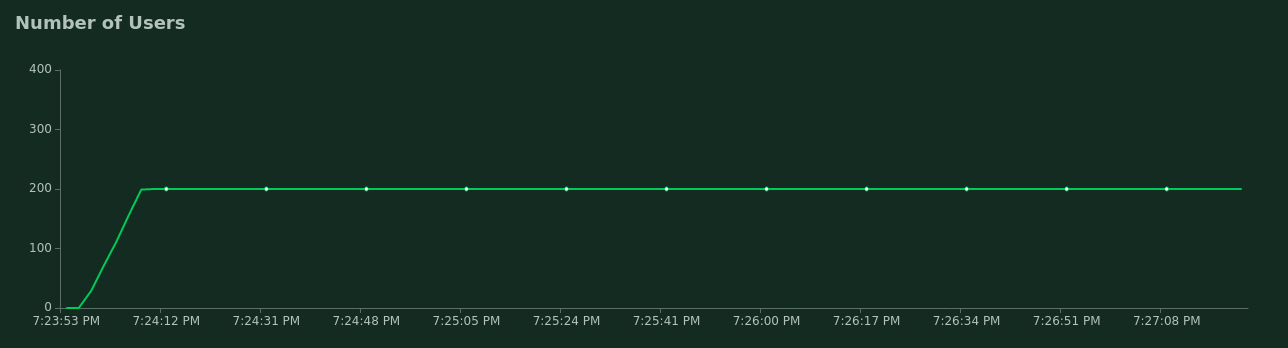
\includegraphics[width=.95\linewidth]{tests/swarm/200/number_of_users_1588271033.png}
  \end{minipage}%
  \label{fig:LocalTests:number_of_users}
  \begin{minipage}{\textwidth}
    \centering
    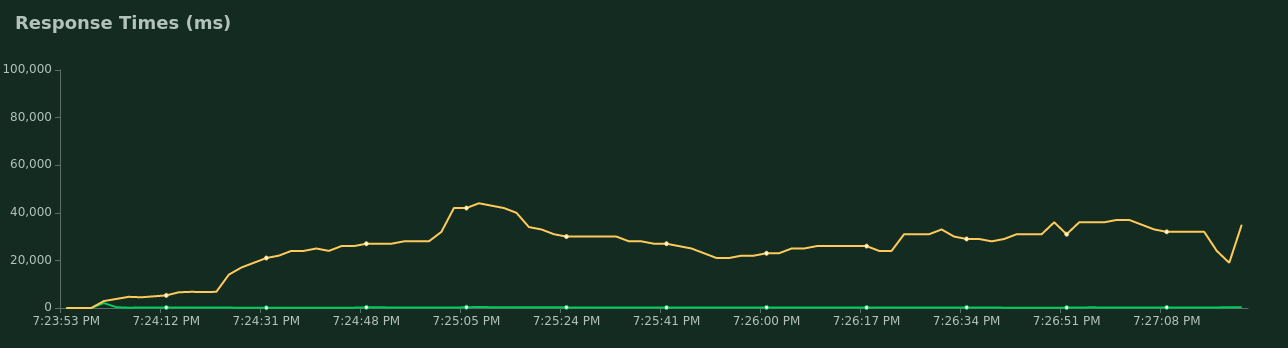
\includegraphics[width=.95\linewidth]{tests/swarm/200/response_times_(ms)_1588271033.png}
  \end{minipage}%
  \label{fig:LocalTests:response_times_(ms)}
  \begin{minipage}{\textwidth}
    \centering
    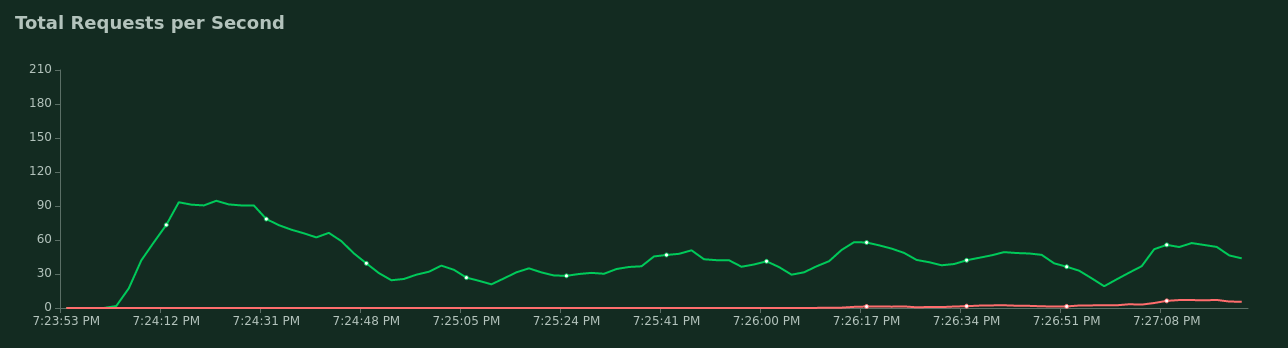
\includegraphics[width=.95\linewidth]{tests/swarm/200/total_requests_per_second_1588271033.png}
  \end{minipage}%
  \caption{Load tests results with 200 users in Docker Swarm.}
  \label{fig:LocalTests:total_requests_per_second}
\end{figure}
\vspace{-10pt}

The closing locust swarm sent an attack of 50 users.
This test was run several times and on average only 16 failed to complete the purchase (with 3 failed attempts).
This seemed to be the fairest amount of users the current infrastructure is able to support simultaneously while providing a reasonable performance.

%%%%%%%%%%%%%%%%%%%%%%%%%%%%%%%%%%%%%%%%

% 50
% 20/s

% Type 	Name 	                                        # Requests 	# Fails   # Exceptions  Median (ms) 	90%ile (ms) 	Average (ms) 	Min (ms) 	Max (ms)
% POST 	/api/v1/organizers/ws/events/ws2020/orders/ 	74 	        46 	      16            2000 	        17000 	      4970 	        425 	    20315
%       Aggregated                                    2341 	      46 	      -             63 	          1500 	        912 	        3 	      32236

%%%%%%%%%%%%%%%%%%%%%%%%%%%%%%%%%%%%%%%%

% 100
% 20/s

% Type 	Name 	                                        # Requests 	# Fails   # Exceptions  Median (ms) 	90%ile (ms) 	Average (ms) 	Min (ms) 	Max (ms)
% POST 	/api/v1/organizers/ws/events/ws2020/orders/ 	202   	    138 	    62            1900 	        18000 	      6003 	        326 	    28477
%       Aggregated                                    5102 	      138 	    -             200 	        8800 	        1974 	        3 	      34930

%%%%%%%%%%%%%%%%%%%%%%%%%%%%%%%%%%%%%%%%

% 200
% 20/s

% Type 	Name 	                                        # Requests 	# Fails   # Exceptions  Median (ms) 	90%ile (ms) 	Average (ms) 	Min (ms) 	Max (ms)
% POST 	/api/v1/organizers/ws/events/ws2020/orders/ 	308 	      243 	    108           5200 	        23000 	      8675 	        295 	    42395 	
%       Aggregated                                    9488 	      243 	    -             180 	        18000 	      3801 	        3 	      63114 	

%%%%%%%%%%%%%%%%%%%%%%%%%%%%%%%%%%%%%%%%

% 250
% 20/s

% Type 	Name 	                                        # Requests 	# Fails   # Exceptions  Median (ms) 	90%ile (ms) 	Average (ms) 	Min (ms) 	Max (ms)
% POST 	/api/v1/organizers/ws/events/ws2020/orders/ 	362 	      239 	    84            1800 	        38000 	      11743 	      274 	    53261
%       Aggregated                                    11925     	297 	    -             170 	        25000 	      4899 	        3 	      90735 	

% postFailures = {500: 7, 409: 84}
% getFailures = {500: 7}

%%%%%%%%%%%%%%%%%%%%%%%%%%%%%%%%%%%%%%%%

% 400
% 20/s

% Type 	Name 	                                        # Requests 	# Fails   # Exceptions  Median (ms) 	90%ile (ms) 	Average (ms) 	Min (ms) 	Max (ms)
% POST 	/api/v1/organizers/ws/events/ws2020/orders/ 	599 	      492 	    178           2000 	        45000 	      12104 	      3 	      60399
%       Aggregated                                    19010 	    1224 	    -             210 	        23000 	      5767 	        3 	      117999 	

% postFailures = {502: 54, 409: 178, 504: 17, 500: 5}
% getFailures = {500: 45, 502: 467, 504: 220}

%%%%%%%%%%%%%%%%%%%%%%%%%%%%%%%%%%%%%%%%


\subsection{Bottlenecks} \label{performance.bottlenecks} %%%%%%%%%%%%%%%%%%%

% what performance bottlenecks were found?

Before presenting our analysis to the results, a few remarks must be presented as well - a sort of pre-analysis.
This allows the reader to greatly understand the external constraints that limited our ability to test the infrastructure and thus influenced our approaches 
when load testing.

The first aspect to consider is how the failures were truly computed.
Locust returns a failed request when the server's response code isn't within 200 and 299, but we noticed a case where this had to be treated differently.
Pretix' documentation states that \texttt{409 Conflict} responses "are intended to be retried" and their occurrence were due to the service's implementation itself.
With a lack of documentation on this, we decided to simplify and for every API request attempt 3 times if the response had that code.
Our counts correspond to this form of error counting.

The second aspect applies to the load tests executed in Docker Swarm mode.
In this scenario the first clear bottleneck was the internet connection between the attacker computer and the department's infrastructure.
This rendered tests invalid and even brought problems to our own computers so it was quickly forgotten as a form of testing.
The alternative was to build containers dedicated to perform the locust swarm and launch them in one of the remote machines available for us and separate from 
the services themselves.
Such adaptation in a way made the test less real, since the physical distance between server and client is practically none, but in another increased realism 
since clients would probably be purchasing tickets from different networks and thus would never saturate the connection to the server like it was occurring with 
our initial tests.

After performing a diagnosis on what could be limiting the infrastructure's performance, we came to a few hypothesis.
The first had to do with the overall connection capacity that was not ideal from the beginning. 
The bandwidth was limited to 100 Mb per second and, with a purchase process as heavy as ours (that implies many data exchanges of invoices, images, etc.), the 
connection could quickly get saturated.
Other factor not directly related to our solution itself was the usage of shared remote resources.
During development many setbacks appeared from external factors such as the used VPN's configuration, and load tests became more frequent amongst developers by 
the end of the delivery date, resulting in far more activity and thus slower responses.
This could be very much connected to the occurrence of the errors of type \texttt{500} or greater. 

Regarding aspects with greater value for our future work, a few conclusions were reached.
First of all, we understood Pretix' service was not optimized to receive as many requests as we initially thought.
This could even be related to an incorrect interpretation from us of the numbers provided by them, i.e. Pretix' authors state the service supports 500 users per 
minute which is about 8 users per second, but our tests had moments where almost twice as many users were finishing their orders.
The way our load tests work, the way locust works, does not allow us to control this and activity peaks always occur, so the results are greatly affected.

Nevertheless we understand that the provided Docker image of Pretix might not be their most refined solution, keeping that one for themselves and their paid 
partnerships.
This could also help explain why so many responses of type \texttt{409 Conflict} are returned, although we were not able to pin point exactly why their 
implementation fosters such responses. 

\newpage
\section{Additional Remarks} \label{remarks} %%%%%%%%%%%%%%%%%%%%%%%%%%%%%%%%%%%%%%%%%%%%%%%%%%%%%%%%%%%%%%%%%%%%%%%%%%%%%%%%%%%%%%%%%%%%%%%%%%%%%%%%%%%%%%%%%%%

\subsection{Pretix Quickstart} \label{remarks.quickstart} %%%%%%%%%%%%%%%%%%

% quickstart script

During development, a need for a faster basic setup of Pretix emerged for debugging purposes.
As many of our tests assumed the existence of organizers and events already inserted on the databases, each time these had to be cleared the objects had to be 
manually created before proceeding with some implementation process.

In order to respond to this need, we developed a Python script capable of completely dispose of the manual labour.
This script, which we called \texttt{quickstart.py} and placed under a dedicated folder, uses Selenium \cite{selenium} to create an organization inside Pretix, 
generate a secret API key for sending REST requests (storing it in a text file), create a default event and prepare it for load testing with Locust.
It also contains configurable variables to personalize its output.

Such quickstart tool was not only found useful for the obvious advantage in development speed it brought to us, but was also considered a good help tool for any 
person that wishes to quickly experiment our infrastructure without having to know much about Pretix itself.

\subsection{Planning Phase 2} \label{remarks.planning} %%%%%%%%%%%%%%%%%%%%%

% what is to be done until the final delivery?
% docker secrets, fault tolerance, 

Providing a service like Pretix proved to be quite a challenge given its complexity, dependencies and considering the quality attributes we were aiming to achieve.
Once our efforts reached solid results, we came to gain deep knowledge about what was truly being provided to clients, what bottlenecks our infrastructure has 
and how it behaves when handling great volumes of requests.
With the gathered information, it is now possible to personalize and optimize the stack for Pretix to achieve a better overall performance.
The basis has been established to proceed towards making the solution more fault tolerant, scalable, reliable and define monitoring strategies.

The goal now is to develop automatic mechanisms that will allow the infrastructure manager to easily deal with traffic fluctuations and handle errors and crashes.
We intend to provide tools that ensure the manager that a service never fails and that allow a quick escalation of the stack according to incoming traffic.
Part has already been tackled so far, namely the implementation of clusters for both of the storage systems necessary for Pretix, which already guarantees 
replication and redundancy of information, and fault tolerance as well, but this is to be improved for the final delivery.

To do this, we intend to develop Ansible scripts that will enable automatic service stack scaling and possibly automatic service crash handling and redeployment.
Ansible \cite{ansible} is an IT automation engine that automates cloud provisioning, configuration management, application deployment, intra-service orchestration 
and many other IT needs, exactly the type of engine we need to further improve our infrastructure.

Additional aspects will be taken in consideration, namely security. 
By injecting any password needed to services through the secrets Docker API we aim to achieve a more secure and penetration resistant system. 
This was already done with configuration files needed to be injected in some of our services, but we intend to extend this process to any critical information 
such as passwords.

Lastly, a monitoring solution will also be implemented, since that is a crucial aspect of any system in production. 
A monitoring platform gives all the feedback and insights necessary for the infrastructure manager to make decisions, such as scale the service stack or 
intervene in a possible security breach or significant bug. 
The framework we intend to use is still being decided, but we already researched and found some options that can suit our scenario.

\subsection{Documentation} \label{remarks.documentation} %%%%%%%%%%%%%%%%%%%

% what documentation was produced?

A great portion of the code we deal with isn't of our authorship, so the documentation it contains is the documentation we get.
Nevertheless, the code we developed has specific purposes and, although usually very much self explanatory due to its nature, should be easy to interpret by any person.
Our goal is to ensure that what we deliver can be easily reused or even continued by other developers.

With this in mind, we made significant efforts on ensuring that all code developed by us followed a common structure with the same coding style.
Also, we made sure all source files have a description of their purpose and relevant information on the first lines, and contain comments on key points of the 
code explaining snippets considered of greater complexity/importance.

\subsection{Assignment Contributions} \label{remarks.contributions} %%%%%%%%

% who did what?

Regarding the work distribution amongst developers, a close-contact strategy was defined where each worked on a cluster component or piece of software according 
to a predefined plan. 
The cluster strategy and respective details were decided in conjunction, as well as the key objectives and tasks to be achieved before the final delivery deadline.

Pretix' features were explored by both developers in order to better comprehend the web platform and the REST API.
Then, João focused on the deployment of our solution on the department's infrastructure while Filipe focused on creating and executing the load tests.
The analysis of the results were carefully conducted in conjunction as well, in order to maintain a common knowledge for better workflows.
It is needless to say that bug and error solving was made along the development phase by both developers any time it was required.
Once performance benchmarking and bottleneck identification were completed, this report and the code documentation became our primary concern, with both 
contributing equally.

\newpage
\section*{Conclusions} \label{conclusions} %%%%%%%%%%%%%%%%%%%%%%%%%%%%%%%%%%%%%%%%%%%%%%%%%%%%%%%%%%%%%%%%%%%%%%%%%%%%%%%%%%%%%%%%%%%%%%%%%%%%%%%%%%%%%%%%%%%%%

The results of our load tests were quite demotivating, since it was understood that Pretix could support much less users we had once expected.
Nevertheless the outcome allowed us to look at the overall solution with different eyes and understand where were we thinking in a not so correct way and where 
were our weak spots, those of Pretix and those of the department's hardware as well.
The bottleneck analysis turned out to be not as conclusive as one could whish for, as they appear to have much to do with Pretix' implementation itself.
To deal with this, some code analysis will have to be executed in parallel to the continuation of the project.

If once we had some questions regarding the complexity of maintaining a service in the cloud, today there is no doubt about the importance of the work of those 
that ensure its correct functioning and constant availability.
Many concepts we had discussed during classes and in prior courses were explored in great depth through this practical hands-on assignment.
And although the difficulties are constant and the challenges are many, we have now reached a point where we are eager to see how far can our solutions go in 
terms of performance and quality. 

We complete this intermediate phase knowing our service in far greater detail when compared to when we started exploring Pretix' features.
With the gathered information, we intend to overcome or at least attenuate its flaws and improve the infrastructure's performance and monitoring capabilities.
Our perspective on the work delivered and here described is very positive, since we were able to configure a complete, redundant, fault-tolerant and maintainable 
infrastructure based on Docker Compose and Swarm with smart strategies such as those within our clusters and useful additions such as the Docker secrets feature.

\newpage
\begin{thebibliography}{9} %%%%%%%%%%%%%%%%%%%%%%%%%%%%%%%%%%%%%%%%%%%%%%%%%%%%%%%%%%%%%%%%%%%%%%%%%%%%%%%%%%%%%%%%%%%%%%%%%%%%%%%%%%%%%%%%%%%%%%%%%%%%%%%%%%%%%
  \bibliographystyle{Science}

  \bibitem{assign}
    J. P. Barraca,
    \textit{GIC - Report no.1: Simple Product Operation},
    University of Aveiro,
    2019/20.
    \vspace{-10pt}

  \bibitem{pretix}
    \textit{About Pretix},
    \url{https://pretix.eu/about/en/}.
    Pretix.eu,
    retrieved in April 2020.
    \vspace{-10pt}

  \bibitem{rami.io}
    \textit{Welcome to Rami.io},
    \url{https://rami.io/}.
    Rami.io,
    retrieved in April 2020.
    \vspace{-10pt}

  \bibitem{pretixgit}
    \textit{Pretix Code Repository},
    \url{https://github.com/pretix/pretix}.
    GitHub, Inc.,
    retrieved in April 2020.
    \vspace{-10pt}

  \bibitem{pretixdoc}
    \textit{Welcome to pretix' documentation!},
    \url{https://docs.pretix.eu/en/latest/}.
    Pretix.eu,
    retrieved in April 2020.
    \vspace{-10pt}

  \bibitem{docker}
    \textit{Docker Homepage},
    \url{https://www.docker.com/}.
    Docker Inc.,
    retrieved in April 2020.
    \vspace{-26pt}

  \bibitem{pretix_img}
    \textit{pretix/standalone},
    \url{https://hub.docker.com/r/pretix/standalone}.
    pretix,
    retrieved in April 2020.
    \vspace{-10pt}

  \bibitem{django}
    \textit{Meet Django},
    \url{https://www.djangoproject.com/}.
    Django Software Foundation and individual contributors,
    retrieved in April 2020.
    \vspace{-10pt}

  \bibitem{gunicorn}
    \textit{Gunicorn Homepage},
    \url{https://gunicorn.org/}.
    Gunicorn.org,
    retrieved in April 2020.
    \vspace{-10pt}

  \bibitem{nginx}
    \textit{NGinX News},
    \url{https://nginx.org/}.
    NGinX.org,
    retrieved in April 2020.
    \vspace{-10pt}

  \bibitem{postgresql}
    \textit{PostgreSQL: The World's Most Advanced Open Source Relational Database},
    \url{https://www.postgresql.org/}.
    The PostgreSQL Global Development Group,
    retrieved in April 2020.
    \vspace{-10pt}

  \bibitem{redis}
    \textit{About Redis},
    \url{https://redis.io/}.
    Redis Labs,
    retrieved in April 2020.
    \vspace{-10pt}

  \bibitem{pgpool}
    \textit{Welcome to Pgpool-II},
    \url{https://www.pgpool.net/mediawiki/index.php/Main_Page}.
    PgPool Global Development Group,
    retrieved in April 2020.
    \vspace{-10pt}

  \bibitem{haproxy}
    \textit{HAProxy: The Reliable, High Performance TCP/HTTP Load Balancer},
    \url{https://www.haproxy.org/}.
    HAProxy.org,
    retrieved in April 2020.
    \vspace{-10pt}

  

  \bibitem{locust}
    \textit{Locust, an open source load testing tool},
    \url{https://locust.io/}.
    Locust.io,
    retrieved in April 2020.
    \vspace{-10pt}

  \bibitem{selenium}
    \textit{About Selenium},
    \url{https://www.selenium.dev/about/}.
    Software Freedom Conservancy,
    retrieved in April 2020.
    \vspace{-10pt}

  \bibitem{ansible}
    \textit{Ansible},
    \url{https://www.ansible.com/}.
    Red Hat,
    retrieved in April 2020.
    

\end{thebibliography}

\clearpage

\end{document}




















